\documentclass[utf8x, 12pt]{G7-32}

% Настройки стиля ГОСТ 7-32
% Для начала определяем, хотим мы или нет, чтобы рисунки и таблицы нумеровались в пределах раздела, или нам нужна сквозная нумерация.
\EqInChapter % формулы будут нумероваться в пределах раздела
\TableInChapter % таблицы будут нумероваться в пределах раздела
\PicInChapter % рисунки будут нумероваться в пределах раздела
\usepackage{slashbox}

\usepackage[table,xcdraw]{xcolor}

% Добавляем гипертекстовое оглавление в PDF
\usepackage[
bookmarks=true, colorlinks=true, unicode=true,
urlcolor=black,linkcolor=black, anchorcolor=black,
citecolor=black, menucolor=black, filecolor=black,
]{hyperref}

% Изменение начертания шрифта --- после чего выглядит таймсоподобно.
% \usepackage{cyrtimespatched}

% графика
\usepackage{graphicx}
\graphicspath{ {./img/} }

% отделять первую строку раздела абзацным отступом
\usepackage{indentfirst} 

% Пакет Tikz
\usepackage{tikz}
\usetikzlibrary{arrows,positioning,shadows}

% Произвольная нумерация списков.
\usepackage{enumerate}

% ячейки в несколько строчек
\usepackage{multirow}

% itemize внутри tabular
\usepackage{paralist,array}

% объявляем новую команду для переноса строки внутри ячейки таблицы
\newcommand{\specialcell}[2][c]{%
	\begin{tabular}[#1]{@{}c@{}}#2\end{tabular}}

\usepackage{tikz}
\usepackage{pgfplots}
\usepackage{pdfpages}
\usepackage{caption}

% \usepackage{extsizes} % Для добавления в параметры класса документа 14pt

% Для работы с несколькими языками и шрифтом Times New Roman по-умолчанию
\usepackage[english,russian]{babel}
% \usepackage{fontspec}
% \setmainfont{Times New Roman}

\usepackage{ulem} % Нормальное нижнее подчеркивание
\usepackage{hhline} % Двойная горизонтальная линия в таблицах
\usepackage[figure,table]{totalcount} % Подсчет изображений, таблиц
\usepackage{rotating} % Поворот изображения вместе с названием
\usepackage{lastpage} % Для подсчета числа страниц

% \captionsetup[table]{position=top}

% Дополнительное окружения для подписей
\usepackage{array}
\newenvironment{signstabular}[1][1]{
	\renewcommand*{\arraystretch}{#1}
	\tabular
}{
	\endtabular
}

% \usepackage[cache=false, newfloat]{minted}

%  Подсчёт числа цитирования
% необходимо скачать и установить (см. readme) https://ctan.org/pkg/totcount
\usepackage{totcount}
\newtotcounter{citnum} %From the package documentation
\def\oldbibitem{} \let\oldbibitem=\bibitem
\def\bibitem{\stepcounter{citnum}\oldbibitem}


% Листинги

\usepackage{listings}
\usepackage{caption}

\usepackage{courier}
\usepackage{wrapfig}

\usepackage{xcolor}
\captionsetup[lstlisting]{singlelinecheck=off, justification=raggedright}


\definecolor{codegreen}{rgb}{0,0.6,0}
\definecolor{codegray}{rgb}{0.5,0.5,0.5}
\definecolor{codepurple}{rgb}{0.58,0,0.82}
\definecolor{backcolour}{rgb}{0.95,0.95,0.92}


% Значения по умолчанию
\lstset{
  % подсветка синтаксиса
  backgroundcolor=\color{backcolour},   
  commentstyle=\color{codegreen},
  keywordstyle=\color{magenta},
  numberstyle=\tiny\color{codegray},
  stringstyle=\color{codepurple},
  basicstyle= \footnotesize,
  breakatwhitespace=true,% разрыв строк только на whitespacce
  breaklines=true,       % переносить длинные строки
%   captionpos=b,          % подписи снизу -- вроде не надо
  inputencoding=koi8-r,
  numbers=left,          % нумерация слева
  numberstyle=\footnotesize,
  showspaces=false,      % показывать пробелы подчеркиваниями -- идиотизм 70-х годов
  showstringspaces=false,
  showtabs=false,        % и табы тоже
  stepnumber=1,
  tabsize=4,              % кому нужны табы по 8 символов?
  frame=single,
  escapeinside={(*}{*)}, %выделение
  literate={а}{{\selectfont\char224}}1
  {б}{{\selectfont\char225}}1
  {в}{{\selectfont\char226}}1
  {г}{{\selectfont\char227}}1
  {д}{{\selectfont\char228}}1
  {е}{{\selectfont\char229}}1
  {ё}{{\"e}}1
  {ж}{{\selectfont\char230}}1
  {з}{{\selectfont\char231}}1
  {и}{{\selectfont\char232}}1
  {й}{{\selectfont\char233}}1
  {к}{{\selectfont\char234}}1
  {л}{{\selectfont\char235}}1
  {м}{{\selectfont\char236}}1
  {н}{{\selectfont\char237}}1
  {о}{{\selectfont\char238}}1
  {п}{{\selectfont\char239}}1
  {р}{{\selectfont\char240}}1
  {с}{{\selectfont\char241}}1
  {т}{{\selectfont\char242}}1
  {у}{{\selectfont\char243}}1
  {ф}{{\selectfont\char244}}1
  {х}{{\selectfont\char245}}1
  {ц}{{\selectfont\char246}}1
  {ч}{{\selectfont\char247}}1
  {ш}{{\selectfont\char248}}1
  {щ}{{\selectfont\char249}}1
  {ъ}{{\selectfont\char250}}1
  {ы}{{\selectfont\char251}}1
  {ь}{{\selectfont\char252}}1
  {э}{{\selectfont\char253}}1
  {ю}{{\selectfont\char254}}1
  {я}{{\selectfont\char255}}1
  {А}{{\selectfont\char192}}1
  {Б}{{\selectfont\char193}}1
  {В}{{\selectfont\char194}}1
  {Г}{{\selectfont\char195}}1
  {Д}{{\selectfont\char196}}1
  {Е}{{\selectfont\char197}}1
  {Ё}{{\"E}}1
  {Ж}{{\selectfont\char198}}1
  {З}{{\selectfont\char199}}1
  {И}{{\selectfont\char200}}1
  {Й}{{\selectfont\char201}}1
  {К}{{\selectfont\char202}}1
  {Л}{{\selectfont\char203}}1
  {М}{{\selectfont\char204}}1
  {Н}{{\selectfont\char205}}1
  {О}{{\selectfont\char206}}1
  {П}{{\selectfont\char207}}1
  {Р}{{\selectfont\char208}}1
  {С}{{\selectfont\char209}}1
  {Т}{{\selectfont\char210}}1
  {У}{{\selectfont\char211}}1
  {Ф}{{\selectfont\char212}}1
  {Х}{{\selectfont\char213}}1
  {Ц}{{\selectfont\char214}}1
  {Ч}{{\selectfont\char215}}1
  {Ш}{{\selectfont\char216}}1
  {Щ}{{\selectfont\char217}}1
  {Ъ}{{\selectfont\char218}}1
  {Ы}{{\selectfont\char219}}1
  {Ь}{{\selectfont\char220}}1
  {Э}{{\selectfont\char221}}1
  {Ю}{{\selectfont\char222}}1
  {Я}{{\selectfont\char223}}1
}

\lstloadlanguages{
  C++
}

% Стиль для псевдокода: строчки обычно короткие, поэтому размер шрифта побольше
\lstdefinestyle{pseudocode}{
  basicstyle=\small,
  keywordstyle=\color{black}\bfseries\underbar,
  language=Pseudocode,
  numberstyle=\footnotesize,
  commentstyle=\footnotesize\it
}

% Стиль для обычного кода: маленький шрифт
\lstdefinestyle{realcode}{
  basicstyle=\scriptsize,
  numberstyle=\footnotesize
}

% Стиль для коротких кусков обычного кода: средний шрифт
\lstdefinestyle{simplecode}{
  basicstyle=\footnotesize,
  numberstyle=\footnotesize
}

% Стиль для BNF
\lstdefinestyle{grammar}{
  basicstyle=\footnotesize,
  numberstyle=\footnotesize,
  stringstyle=\bfseries\ttfamily,
  language=BNF
}

% Определим свой язык для написания псевдокодов на основе Python
\lstdefinelanguage[]{Pseudocode}[]{Python}{
  morekeywords={each,empty,wait,do},% ключевые слова добавлять сюда
  morecomment=[s]{\{}{\}},% комменты {а-ля Pascal} смотрятся нагляднее
  literate=% а сюда добавлять операторы, которые хотите отображать как мат. символы
    {->}{\ensuremath{$\rightarrow$}~}2%
    {<-}{\ensuremath{$\leftarrow$}~}2%
    {:=}{\ensuremath{$\leftarrow$}~}2%
    {<--}{\ensuremath{$\Longleftarrow$}~}2%
}[keywords,comments]

% Свой язык для задания грамматик в BNF
\lstdefinelanguage[]{BNF}[]{}{
  morekeywords={},
  morecomment=[s]{@}{@},
  morestring=[b]",%
  literate=%
    {->}{\ensuremath{$\rightarrow$}~}2%
    {*}{\ensuremath{$^*$}~}2%
    {+}{\ensuremath{$^+$}~}2%
    {|}{\ensuremath{$|$}~}2%
}[keywords,comments,strings]

% Подписи к листингам на русском языке.
\renewcommand\lstlistingname{\cyr\CYRL\cyri\cyrs\cyrt\cyri\cyrn\cyrg}
\renewcommand\lstlistlistingname{\cyr\CYRL\cyri\cyrs\cyrt\cyri\cyrn\cyrg\cyri}

% \usepackage{enumitem}
% \setlist[itemize]{itemsep=10pt, label={--}}

% ---------------------- Документ ----------------------
\begin{document}

	\frontmatter % выключает нумерацию ВСЕГО; здесь начинаются ненумерованные главы: реферат, введение, глоссарий, сокращения и прочее.

		\noindent\begin{minipage}{0.05\textwidth}
		
\includegraphics[scale=0.3]{bmstu.png}
	\end{minipage}
	\hfill
	\begin{minipage}{0.85\textwidth}\raggedleft
		\begin{center}
			\fontsize{12pt}{0.3\baselineskip}\selectfont \textbf{Министерство науки и высшего образования Российской Федерации \\ Федеральное государственное бюджетное образовательное учреждение \\ высшего образования \\ <<Московский государственный технический университет \\ имени Н.Э. Баумана \\ (национальный исследовательский университет)>> \\ (МГТУ им. Н.Э. Баумана)}
		\end{center}
	\end{minipage}

	\begin{center}
		\fontsize{12pt}{0.1\baselineskip}\selectfont
		\noindent\makebox[\linewidth]{\rule{\textwidth}{4pt}} \makebox[\linewidth]{\rule{\textwidth}{1pt}}
	\end{center}

	\begin{flushleft}
		\fontsize{12pt}{0.8\baselineskip}\selectfont 
		
		ФАКУЛЬТЕТ \uline{<<\textbf{Информатика и системы управления}>> \hfill}

		КАФЕДРА \uline{\mbox{\hspace{4mm}} <<\textbf{Программное обеспечение ЭВМ и информационные технологии}>> \hfill}
	\end{flushleft}

	\vfill

	\begin{center}
		\fontsize{20pt}{\baselineskip}\selectfont

		\textbf{РАСЧЕТНО-ПОЯСНИТЕЛЬНАЯ ЗАПИСКА}

		\textbf{\textit{К КУРСОВОЙ РАБОТЕ}}

		\textbf{\textit{НА ТЕМУ:}}
	\end{center}

	\begin{center}
		\fontsize{18pt}{0.6cm}\selectfont 
		
		<<Мониторинг системных вызовов в ОС Linux>>
		
	\end{center}

	\vfill

	\begin{table}[h!]
		\fontsize{12pt}{0.7\baselineskip}\selectfont
		\centering
		\begin{signstabular}[0.7]{p{7.25cm} >{\centering\arraybackslash}p{4cm} >{\centering\arraybackslash}p{4cm}}
			Студент группы ИУ7-75Б & \uline{\mbox{\hspace*{4cm}}} & \uline{\hfill М.А. Козлов \hfill} \\
			& \scriptsize (Подпись, дата) & \scriptsize (И.О. Фамилия)
		\end{signstabular}

		\vspace{\baselineskip}

		\begin{signstabular}[0.7]{p{7.25cm} >{\centering\arraybackslash}p{4cm} >{\centering\arraybackslash}p{4cm}}
			Руководитель курсового проекта & \uline{\mbox{\hspace*{4cm}}} & \uline{\hfill Н. Ю. Рязанова \hfill} \\
			& \scriptsize (Подпись, дата) & \scriptsize (И.О. Фамилия)
		\end{signstabular}

		\vspace{\baselineskip}
	\end{table}

	\vfill

	\begin{center}
		\normalsize \textit{\textbf{2021} г.}
	\end{center}

	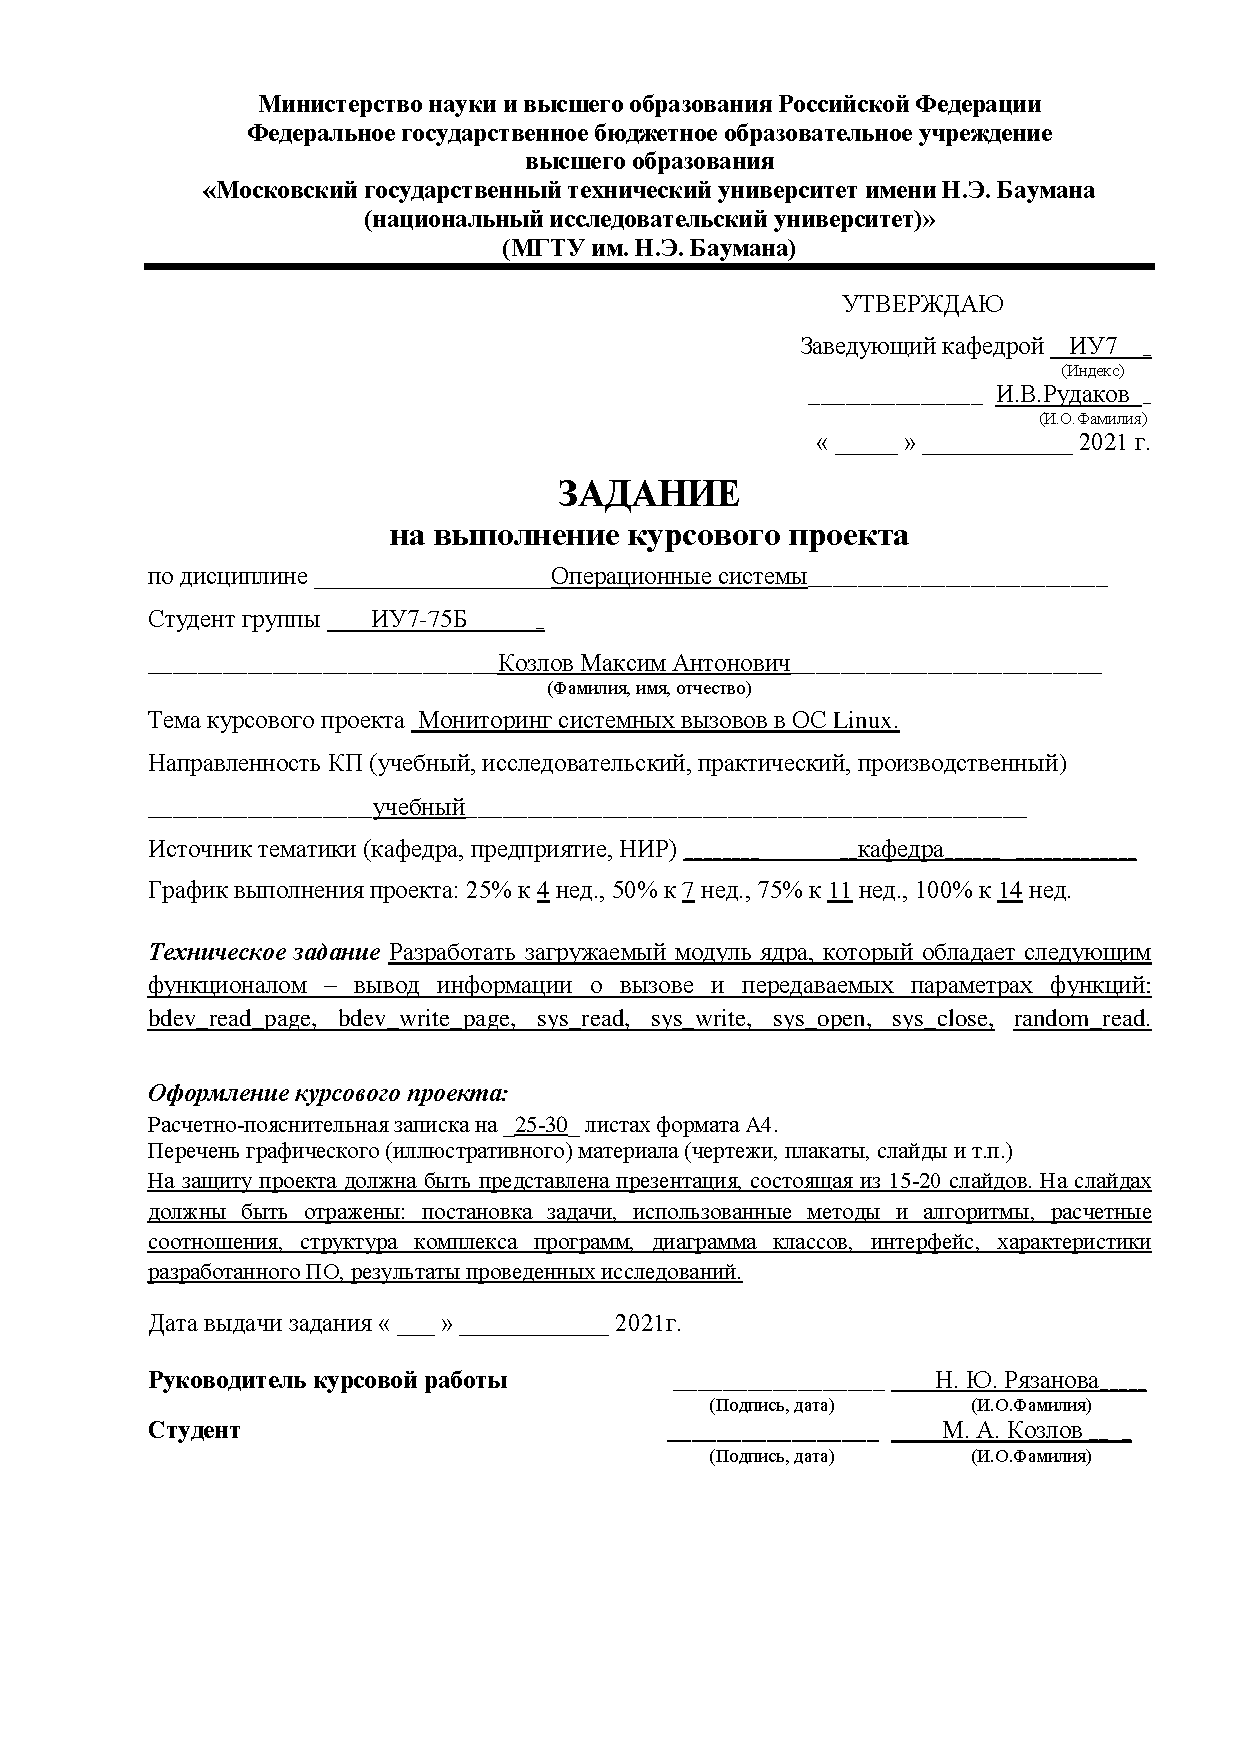
\includepdf{TZ_Kozlov.pdf}

	\renewcommand{\contentsname}{\normalsize\bfseries\centering СОДЕРЖАНИЕ}
	\small
	\tableofcontents
	\normalsize

	\pagebreak
	
	\Introduction
    Одна из актуальных задач мониторинга операционных систем является
    мониторинг системных вызовов для выявления узких мест и исследования особенностей её работы.
    В операционных системах семейства Linux
    это можно реализовать с помощью загружаемых модулей ядра,
    используя различные методы перехвата системных вызовов,
    которые будут описаны в аналитическом разделе.

    Целью курсовой работы является разработка загружаемого модуля ядра,
    позволяющего логировать вызов следующих функций: 
    bdev\_read\_page, 
    bdev\_write\_page, 
    sys\_read, sys\_write, 
    sys\_open, 
    sys\_close, 
    random\_read.

\pagebreak

	\mainmatter % это включает нумерацию глав и секций в документе ниже

	\chapter{Аналитический раздел}
	\section{Постановка задачи}
		В соответствии с заданием на курсовую работу
		необходимо разработать загружаемый модуль ядра,
	 	позволяющий перехватывать системные вызовы:
		bdev\_read\_page,
		bdev\_write\_page,
		sys\_read,
		sys\_write,
		sys\_open,
		sys\_close,
		random\_read и выводить в системный журнал информацию о 
		идентификаторе вызывающего процесса, 
		передаваемых параметрах и возвращаемого значения.

		Для достижения поставленной цели требуется решить следующие задачи:
		\begin{enumerate}
			\item проанализировать перехватываемые функции;
			\item проанализировать существующие способы перехвата функций;
			\item реализовать загружаемый модуль ядра;
			\item исследовать поведение перехваченных функций.
		\end{enumerate}
	
	\section{Анализ перехватываемых системных вызовов}
		Перехватываемые системные функции позволяют 
		отслеживать работу системы относительно 
		основных операций по работе с файловыми системами,
		а также связанных с символьными и блочными устройствами.

		Сигнатуры данных функций зависят от версии ядра Linux, 
		поэтому будет реализована поддержка только версии ядра 5.0.
		Все дальнейшие структуры и функции ядра приведены для данной версии ядра, 
		если явно не указана иная.
		
	\subsection*{Анализ системного вызова bdev\_read\_page}
		Функция bdev\_read\_page имеет следующую сигнатуру \cite{linux-bdev_read_page}:\\
		\lstinline{int bdev_read_page(struct block_device *bdev, sector_t sector, struct page *page)},

		где \lstinline{struct block_device *bdev} -- блочное устройство с которого считывается информация,

		\lstinline{sector_t sector} -- смещение на устройстве для чтения страницы,
		
		\lstinline{struct page *page} -- страница для записи считанных данных.

		Данная функция начинает операцию чтения страницы с блочного устройства, 
		блокируя страницу на время выполнения.
		Ошибки возвращаемые этой функцией (отрицательный \lstinline{errno}), обычно <<мягкие>>, 
		т.е. существуют альтернативные способы чтения данных с устройства и
		не требуется распространять ошибку вверх по стеку вызовов.

	 \subsection*{Анализ системного вызова bdev\_write\_page}
		Функция bdev\_write\_page имеет следующую сигнатуру \cite{linux-bdev_write_page}:\\
		\lstinline{int bdev_write_page(struct block_device *bdev, sector_t sector, struct page *page, struct writeback_control *wbc)},
		
		где \lstinline{struct block_device *bdev} -- блочное устройство для записи страницы,

		\lstinline{sector_t sector} -- смещение на устройстве на которое будет записана страница,

		\lstinline{struct page *page} -- страница с записываемыми данными,

		\lstinline{struct writeback_control * wb} -- управляющая структура, которая сообщает коду обратной записи, как производиться запись.
		
		Функция начинает операцию записи страницы на блочное устройство, блокируя страницу на время выполнения.
		Обработка ошибок, возвращаемых данной функцией аналогична bdev\_read\_page.

	\subsection*{Анализ системного вызова sys\_open}
		Системный вызов sys\_open открывает файл по переданному символьному имени filename.
	    Данная функция имеет следующую сигнатуру \cite{linux-sys_open}: \\
		\lstinline{SYSCALL_DEFINE3(open, const char __user *, filename, int, flags, umode_t, mode)}.

	   Возвращаемое значение open() -- это дескриптор файла, неотрицательное целое число, 
	   которое является индексом записи в таблица дескрипторов открытых файлов.
	   Используя различные флаги можно изменить поведение open().
	   Например, если файл не был найден и указан флаг O\_CREAT, 
	   то будет создан новый файл с указанным именем.

	 \subsection*{Анализ системного вызова sys\_read}
	 	Системный вызов sys\_read считывает из файла, 
		на который ссылается файловый дескриптор fd,
		count байт и записывает их в buf -- буфер из пространства пользователя.
		Данная функция имеет следующую сигнатуру \cite{linux-sys_read}: \\
		\lstinline{SYSCALL_DEFINE3(read, unsigned int, fd, char __user *, buf, size_t, count)}.

		Операция чтения начинается со смещения указанного в struct file, 
		после чего смещение файла увеличивается на число прочитанных байтов. 
		Если смещение файла находится в конце или больше конца файла,
		байты не читаются, а read возвращает ноль.

	 \subsection*{Анализ системного вызова sys\_write}
		Системный вызов sys\_write записывает в файл, 
		на который ссылается файловый дескриптор fd,
		count байтов из буфера buf -- буфера пространства пользователя.
		Данная функция имеет следующую сигнатуру \cite{linux-sys_write}: \\
	 	\lstinline{SYSCALL_DEFINE3(write, unsigned int, fd, const char __user *, buf, size_t, count)}.

		Операция записи происходит в файл с указанного смещение,
		а смещение файла увеличивается на количество записанных байтов.
		Если файл был открыт с флагом O\_APPEND, 
		смещение файла сначала устанавливается на конец файла перед записью.
       	Регулировка смещения файла и операция записи выполняется как атомарный шаг.

	 \subsection*{Анализ системного вызова sys\_close}
	 	Системный вызов sys\_close закрывает файл, на который ссылается файловый дескриптор fd, освобождая ресурсы.
		Данная функция имеет следующую сигнатуру \cite{linux-sys_close}: \\
	 	\lstinline{SYSCALL_DEFINE1(close, unsigned int, fd)}.

	 \subsection*{Анализ системного вызова random\_read}
	 	Функция random\_read позволяет считывать массив байт из символьного 
		устройства /dev/random и имеет следующую сигнатуру \cite{linux-random_read}: 
	 \lstinline{static ssize_t random_read(struct file *file, char __user *buf, size_t nbytes, loff_t *ppos)}.
		
	 	Символьное устройство /dev/random генерирует случайные последовательности байт, 
		используя в качестве источника энтропии CSPRNG (криптографически безопасного генератора псевдослучайных чисел).
		Существует похожая функция \lstinline{static ssize_t urandom_read(struct file *file, char __user *buf, size_t nbytes, loff_t *ppos)},
		считывающая данные из символьного устройства 
		/dev/urandom которое отличающается от /dev/random лишь тем, что
		когда энтропия останавливается, он продолжает генерировать последовательности байт. 

\section{Анализ способов перехвата системных вызовов}
	% Под трассировкой понимается получение информации о том, 
	% что происходит внутри работающей системы. 
	% Для этого используются специальные программные инструменты,
	% регистрирующие все события в системе. 
	% Рассмотрим существующие методы перехвата системных вызовов, 

	\subsection*{Linux Security API}
		Linux Security API -- это специальный интерфейс, позволяющий трассировать ядро линукса начиная с версии 2.6 \cite{lsm}.
		В критических местах кода ядра расположены вызовы security-функций, которые в свою очередь вызывают коллбэки,
		установленные security-модулем.
		Security-модуль может изучать контекст операции и принимать решение о её разрешении или запрете.

		Linux Security API имеет ряд ограничений:
		\begin{enumerate}
			\item security-модули не могут быть загружены динамически, являются частью ядра и требуют его пересборки;
			\item в системе может быть только один security-модуль (с небольшими исключениями).
		\end{enumerate}

		Если по поводу множественности модулей позиция разработчиков ядра неоднозначная, 
		то запрет на динамическую загрузку принципиальный: security-модуль должен быть частью ядра,
		чтобы обеспечивать безопасность постоянно, с момента загрузки. 
		Таким образом, для использования Security API необходимо поставлять собственную сборку ядра,
		а также интегрировать дополнительный модуль с SELinux или AppArmor, 
		которые используются популярными дистрибутивами.

	\subsection*{Модификация таблицы системных вызовов}
		В Linux все обработчики системных вызовов хранятся в таблице sys\_call\_table \cite{linux-syscall-reference}.
		Подмена значений в этой таблице приводит к смене поведения всей системы. 
		Таким образом, сохранив старое значения обработчика и подставив в таблицу собственный обработчик, 
		можно перехватить любой системный вызов.

		У этого подхода есть определённые преимущества:
		\begin{enumerate}
			\item Полный контроль над любыми системными вызовами.
				Используя его можно гарантировать перехват действия,
				выполняемого пользовательским процессом.
			\item Минимальные накладные расходы.
				Обновление таблицы системных вызовов происходит один раз при загрузке и выгрузки модуля.
				Помимо полезной нагрузки мониторинга, единственным дополнительным расходом является лишний вызов 
				оригинального обработчика системного вызова.
			\item Минимальные требования к версии ядра.
				Системные таблицы используются в любом ядре Линукса. 
				Однако в новых версиях ядра для передачи аргументов в системные функции
				используются struct pt\_regs. 
				Но данную проблему можно решить, используя условную компиляцию и макрос LINUX\_VERSION\_CODE.
		\end{enumerate}
		
		Однако модификация таблицы системных вызовов не лишена недостатков:
		\begin{enumerate}
			\item Техническая сложность реализации.
				Для замены указателей системных функций в таблице необходимо решить следующие задачи:
				\begin{enumerate}
					\item поиск таблицы системных вызовов;
					\item обход защиты от модификации таблицы;
					\item атомарное и безопасное выполнение замены указателей.
				\end{enumerate}
			
			\item Невозможность перехвата некоторых обработчиков. 
				В ядрах до версии 4.16 обработка системных вызовов для архитектуры x86\_64 содержала целый ряд оптимизаций.
				Некоторые из них требовали того, что обработчик системного вызова реализовались на ассемблере. 
				Соответственно, подобные обработчики порой сложно, а иногда и вовсе невозможно заменить на свои, написанные на Си \cite{habr-ftrace}.
				Более того, в разных версиях ядра используются разные оптимизации, что добавляет различные технические сложности.

			\item Перехватываются только системные вызовы.
				Данный подход позволяет подменить таблицу системных вызовов,
				но это ограничивает количество функций, которые можно мониторить.
		\end{enumerate}
	
	\subsection*{Kprobes}
		Kprobes -- специализированное API, в первую очередь предназначенного для отладки и трассирования ядра \cite{kprobes}.
		Этот интерфейс позволяет устанавливать пред- и пост- обработчики для любой инструкции в ядре,
		а также обработчики на вход и возврат из функции. 
		Обработчики получают доступ к регистрам и могут их изменять. 
		Таким образом, можно было бы получить как мониторинг, так и возможность влиять на дальнейший ход работы.

		Преимущества, которые даёт использование kprobes для перехвата:
		\begin{enumerate}
			\item Обладает хорошо задокументированным интерфейсом, 
				большинство подводных камней уже найдено,
				их работа по возможности оптимизирована.
			\item Перехват любого места в ядре. 
				Kprobes реализуются с помощью точек останова (инструкции int3), 
				внедряемых в исполнимый код ядра. 
				Это позволяет устанавливать kprobes в буквально любом месте любой функции, если оно известно.
				Аналогично, kretprobes реализуются через подмену адреса возврата на стеке и позволяют перехватить
				возврат из любой функции (за исключением тех, которые управление в принципе не возвращают).
		\end{enumerate}
		
		Недостаткам kprobes являются:
		\begin{enumerate}
			\item Техническая сложность. 
				Kprobes -- это только способ установить точку останова в любом места ядра. 
				Для получения аргументов функции или значений локальных переменных надо знать,
				в каких регистрах или где на стеке они лежат, и самостоятельно их оттуда извлекать.
				Для блокировки вызова функции необходимо вручную модифицировать состояние процесса так,
				чтобы процессор подумал, что он уже вернул управление из функции.

			\item Jprobes объявлены устаревшими. 
				Jprobes -- это надстройка над kprobes, позволяющая удобно перехватывать вызовы функций.
				Она самостоятельно извлечёт аргументы функции из регистров или стека и вызовет ваш обработчик,
				который должен иметь ту же сигнатуру, что и перехватываемая функция. 
				Проблема заключается в том, что jprobes объявлены устаревшими и вырезаны из современных ядер
				(начиная с версия 3.19).

			\item Нетривиальные накладные расходы. 
				Расстановка точек останова дорогая, но она выполняется единоразово. 
				Точки останова не влияют на остальные функции, однако их обработка относительно недешёвая.
				Для архитектуры x86\_64 реализована jump-оптимизация, существенно уменьшающая стоимость kprobes,
				но она всё ещё остаётся больше, чем, например, при модификации таблицы системных вызовов.

			\item Ограничения kretprobes. 
				Kretprobes реализуются через подмену адреса возврата на стеке. 
				Соответственно, им необходимо где-то хранить оригинальный адрес,
				чтобы вернуться туда после обработки kretprobe. 
				Адреса хранятся в буфере фиксированного размера. 
				В случае его переполнения, когда в системе выполняется слишком много одновременных вызовов перехваченной функции, 
				kretprobes будет пропускать срабатывания.

			\item Отключенное вытеснение. 
				Kprobes основывается на прерываниях и может менять значения в регистрах процессора,
				следовательно для синхронизации все обработчики выполняются с отключенным вытеснением (preemption).
				Это накладывает определённые ограничения на обработчики: 
				в них нельзя ждать -- выделять много памяти, заниматься вводом-выводом, 
				спать в таймерах и семафорах, и прочее.
		\end{enumerate}

	\subsection*{Kernel tracepoints}
		Kernel tracepoints -- это фреймворк для трассировки ядра, 
		сделанный через статическое инструментирование кода \cite{linux-kernel-tracepoints}.
		Точка трассировки, помещенная в код, обеспечивает ловушку для вызова функции (зонда),
		которую можно предоставить во время выполнения. 
		Точка трассировки может быть "включена" (к ней подключен зонд) или "выключена" (зонд не подключен).
		Когда точка трассировки выключена, она не оказывает никакого эффекта, 
		за исключением проверки условия для перехода и добавлением нескольких байтов для вызова функции 
		в конце инструментированной функции и добавление данных структуру в отдельный раздел.
		Когда точка трассировки включена, предоставляемая функция вызывается каждый раз при выполнении точки трассировки
		в контексте выполнения вызывающей стороны.

		Точки трассировки можно раместить в важных местах кода. 
		Это легкие обработчики, которые могут передавать произвольное количество параметров,
		прототипы которых описаны в объявлении точки трассировки, помещенном в файл заголовка.
		В основном они используются для отслеживания и учета производительности.
		
		Преимуществами данного способа являются:
		\begin{enumerate}
			\item Малые накладные расходы на внедрение в загружаемые модули ядра.
				Необходимо только вызвать функцию трассировки в необходимом месте.

			\item Маленькие затраты по памяти и процессорному времени.
		\end{enumerate}

		Недостатками данного подхода являются:
		\begin{enumerate}
			\item Имена точек трассировки являются глобальными для ядра. 
			Они считаются одинаковыми независимо от того, находятся ли они в ядре или в загружаемых модулях.
			\item Для добавления точек остановки в ядровые функции необходимо перекомпилировать ядро,
			если для данных функций не данные точки не определенны.
			\item Относительно плохо задокументированное API.
		\end{enumerate}
		
	\subsection*{Сплайсинг}
		Сплайсинг -- способ перехвата функций, заключающийся в замене инструкций в начале функции
		на безусловный переход, ведущий в обработчик \cite{splice-hooking}. 
		Оригинальные инструкции переносятся в другое место и исполняются перед переходом обратно в перехваченную функцию.
		С помощью двух переходов вшивается (splice in) дополнительный код в функцию, поэтому такой подход называется сплайсингом.
		Именно таким образом и реализуется jump-оптимизация для kprobes. 
		Используя сплайсинг можно добиться тех же результатов, но без дополнительных расходов на kprobes и с полным контролем ситуации.
		
		Преимуществами сплайсинга являются:
		\begin{enumerate}
			\item Минимальные требования к ядру. 
				Сплайсинг не требует каких-либо особенных опций в ядре и работает в начале любой функции, 
				необходимо лишь знать её адрес.
			\item Минимальные накладные расходы. 
				Два безусловных перехода, которые надо выполнить перехваченному коду, чтобы передать управление обработчику и обратно.
				Подобные переходы отлично предсказываются процессором и являются очень дешёвыми.
			\item Менее заметны для детекторов вредоносных программ.
			\item Позволяет подключать все доступные символы в ядре.
		\end{enumerate}
		
		Недостатками данного подхода являются:
		\begin{enumerate}
			\item Требования к надёжному метод дизассемблерования кода ядра.
			\item Зависимость от архитектуры, поскольку каждая архитектура имеет свои собственные инструкции перехода.
			\item Большая техническая сложность реализации. Ниже приведён краткий и неполный список задач, которые необходимо решить:
			\begin{enumerate}
				\item синхронизация установки и снятия перехвата;
				\item обход защиты от модификации областей памяти с исходным кодом ядра;
				\item инвалидация кешей процессора после замены инструкций;
				\item дизассемблирование заменяемых инструкций, чтобы скопировать их целыми;
				\item проверка на отсутствие переходов внутрь заменяемого куска;
				\item проверка на возможность переместить заменяемый кусок в другое место;
			\end{enumerate}
		\end{enumerate}

	\subsection*{Ftrace}
		Ftrace -- это фреймворк для трассирования ядра на уровне функций \cite{ftrace}.
		Его можно использовать для отладки или анализа задержек и проблем с производительностью, 
		возникающих за пределами пользовательского пространства.

		Хотя ftrace обычно считается трассировщиком функций, 
		на самом деле это структура из нескольких различных утилит трассировки. 
		Имеется трассировка задержки для изучения того, 
		что происходит между отключенными и включенными прерываниями, 
		а также для вытеснения и с момента пробуждения задачи до фактического запланированного выполнения задачи.
		
		Реализуется ftrace на основе ключей компилятора -pg и -mfentry, 
		которые вставляют в начало каждой функции вызов специальной трассировочной функции 
		mcount() или \_\_fentry\_\_(). 
		Обычно, в пользовательских программах эта возможность компилятора используется профилировщиками,
		чтобы отслеживать вызовы всех функций. Ядро же использует эти функции для реализации фреймворка ftrace.

		Вызов ftrace не является дешёвой операцией,
		поэтому для популярных архитектур доступна оптимизация: динамический ftrace. 
		Суть заключается в том, что ядро знает расположение всех вызовов mcount() или \_\_fentry\_\_() 
		и на ранних этапах загрузки заменяет их машинный код на nop -- специальную ничего не делающую инструкцию. 
		При включении трассирования в нужные функции вызовы ftrace добавляются обратно. 
		Таким образом, если ftrace не используется, то его влияние на систему минимально.

		Достоинствами ftrace являются:
		\begin{enumerate}
			\item Использование готовых интерфейсов в ядре существенно упрощает код. 
				Вся установка перехвата требует пары вызовов функций и заполнение двух полей в структуре.
			\item Перехват любой функции по имени. 
				Для указания интересующей нас функции достаточно написать её имя в обычной строке. 
				Не требуются большой разбор внутренних структур данных ядра, сканирование памяти, или дизассемблерования кода ядра.
				Можно перехватить любую функцию (даже не экспортируемую для модулей), зная лишь её имя.
			\item Перехват совместим с трассировкой.
				Данный способ не конфликтует с ftrace,
				так что с ядра можно снимать полезные показатели производительности. 
				Однако использование kprobes или сплайсинга может помешать механизмам ftrace.
			\item Средние накладные расходы. 
				Накладные расходы на ftrace меньше, чем у kprobes (так как ftrace не использует точки останова),
				но они выше, чем у сплайсинга, сделанного вручную. 
				В действительности динамический ftrace является сплайсингом, только дополнительно выполняющий код ftrace и другие коллбеки.
		\end{enumerate}

		Недостатками данного подхода являются:
		\begin{enumerate}
			\item Требования к конфигурации ядра. 
			Для успешного выполнения перехвата функций с помощью ftrace ядро должно предоставлять целый ряд возможностей:
			\begin{enumerate}
				\item список символов kallsyms для поиска функций по имени;
				\item фреймворк ftrace для выполнения трассировки;
				\item различные опции ftrace важные для перехвата.
			\end{enumerate}
			\item Оборачивание функции целиком. 
				Как и сплайсинг, данный подход полностью оборачивает вызовы функций.
				Однако, если сплайсинг технически возможно выполнить в любом месте функции,
				то ftrace срабатывает исключительно при входе. 
				Естественно, обычно это не вызывает сложностей и даже наоборот удобно,
				но подобное ограничение иногда может быть недостатком.
		\end{enumerate}

\section{Сравнительный анализ методов трассировки ядра}
	В таблице \ref{table:compare:hooking} приведено сравнение рассмотренных методов перехвата системных вызовов.
	\begin{table}[h!]
		\caption{Сравнение существующих методов трассировки ядра.}
		\centering
		\begin{tabular}{|c|c|c|c|c|c|c|}
			\hline
			Критерий                                                              & \begin{tabular}[c]{@{}c@{}}Linux \\ Security\end{tabular}      & \begin{tabular}[c]{@{}c@{}}Модификация\\ syscall table\end{tabular} & Kprobes                                                        & \begin{tabular}[c]{@{}c@{}}Kernel\\ tracepoints\end{tabular}   & Сплайсинг                                                      & Ftrace                                                                   \\ \hline
			\begin{tabular}[c]{@{}c@{}}Накладные\\ расходы\end{tabular}           & Средние                                                        & \begin{tabular}[c]{@{}c@{}}Мини-\\ мальные\end{tabular}             & Большие                                                        & Малые                                                          & \begin{tabular}[c]{@{}c@{}}Мини-\\ мальные\end{tabular}        & Средние                                                                  \\ \hline
			\begin{tabular}[c]{@{}c@{}}Сложность\\ реализации\end{tabular}        & Средняя                                                        & Средняя                                                             & Большая                                                        & Средняя                                                        & \begin{tabular}[c]{@{}c@{}}Очень\\ большая\end{tabular}        & Малая                                                                    \\ \hline
			\begin{tabular}[c]{@{}c@{}}Требуется\\ компиляция\\ ядра\end{tabular} & Да                                                             & Нет                                                                 & Иногда                                                         & Иногда                                                         & Нет                                                            & Нет                                                                      \\ \hline
			\begin{tabular}[c]{@{}c@{}}Возможности\\ мониторинга\end{tabular}     & \begin{tabular}[c]{@{}c@{}}Ряд\\ функции\end{tabular}          & \begin{tabular}[c]{@{}c@{}}Системные\\ функции\end{tabular}         & \begin{tabular}[c]{@{}c@{}}Любое\\ место\\ в ядре\end{tabular} & \begin{tabular}[c]{@{}c@{}}Любое\\ место\\ в ядре\end{tabular} & \begin{tabular}[c]{@{}c@{}}Любое\\ место\\ в ядре\end{tabular} & \begin{tabular}[c]{@{}c@{}}Большинство\\ функции\\ по имени\end{tabular} \\ \hline
			\begin{tabular}[c]{@{}c@{}}Докумен-\\ тация\end{tabular}              & Средняя                                                        & Средняя                                                             & Средняя                                                        & Малая                                                          & Малая                                                          & Большая                                                                  \\ \hline
			\begin{tabular}[c]{@{}c@{}}Требования\\ к ядру\end{tabular}           & \begin{tabular}[c]{@{}c@{}}Версия \\ старше\\ 2.6\end{tabular} & Нет                                                                 & \begin{tabular}[c]{@{}c@{}}Версия \\ старше\\ 2.0\end{tabular} & -                                                              & Нет                                                            & \begin{tabular}[c]{@{}c@{}}Наличие\\ ftrace\end{tabular}                 \\ \hline
			\end{tabular}
		\label{table:compare:hooking}
	\end{table}

	Анализируя данную таблицу можно сделать вывод, 
	что для решения поставленной задачи наиболее 
	подходящими являются методы модификации таблицы 
	системных функций и ftrace, т.к. они не требуют
	перекомпиляции ядра и поддерживаются большинством версий ядер,
	а также не вызывают большой технической сложности в реализации.

\section{Выводы}
	В результате анализа работы операционной системы Linux
	с файловыми системами были определены необходимые для мониторинга функции, 
	которые позволят исследовать особенности работы ядра с файлами.

	В результате сравнительного анализа методов перехвата было выбрано два метода.
	Первый метод -- метод модификации таблицы системных вызовов sys\_call\_table
	позволит перехватывать вызовы системных функции sys\_read, sys\_write, sys\_open и sys\_close 
	без больших накладных расходов. 
	Второй -- используя библиотеку ftrace, 
	которая позволит перехватывать функции bdev\_read\_page, bdev\_write\_page и random\_read, 
	т.к. они не определены в таблице sys\_call\_table.

	Выбранные методы перехвата требуют, 
	чтобы сигнатуры перехватываемой функций и функции-перехватчика должны в точности совпадать.
	Иначе, очевидно, аргументы будут переданы неправильно и дальнейшее поведение ядра не определено.
	Из-за этого возникают сложности с поддержкой разных версий ядер Линукса,
	т.к. разработчики ядра не поддерживают обратную совместимость.
	В рамках курсовой работы будет реализована поддержка лишь одной версии ядра -- 5.0.

	% В ходе анализа приведенных подходов к перехвату функций,
	% были выбраны метод модификации таблицы системных вызовов sys\_call\_table и фреймворк ftrace, 
	% так как первый позволит перехватить вызов системных функции sys\_read, sys\_write, sys\_open и sys\_close 
	% без больших накладных расходов.
	% Второй же метод будет 
	% Основными критериями выбора были необходимость перекомпилировать ядро,
	% требования к ядру, а также сложность программной реализации.

	

% \section{Загружаемые модули ядра Linux}
% 	Linux является динамическим ядром, 
% 	поддерживающим добавление и удаление программных компонентов на лету \cite{anatomy-linux-kernel}.
% 	Это означает, есть возможность добавить функциональность в ядро (и убрать её), когда система запущена и работает.
% 	Они называются динамически загружаемыми модулями ядра.
% 	Ядро Linux предлагает поддержку довольно большого числа типов (или классов) модулей.
% 	Каждый модуль является подготовленным объектным кодом (не слинкованным для самостоятельной работы),
% 	который может быть динамически подключен в работающее ядро, а позднее может быть выгружен из ядра.
% 	Каждый модуль ядра регистрирует себя для того, чтобы обслуживать в будущем запросы,
% 	и его функция инициализации немедленно прекращается. 
% 	Иными словами, задача функции инициализации модуля заключается в подготовке функций модуля для последующего вызова.
% 	Функция выхода модуля вызывается только непосредственно перед выгрузкой модуля. 
% 	Функция выхода модуля должна тщательно отменить все изменения, сделанные функцией инициализации, 
% 	или функции модуля сохранятся до перезагрузки системы. 
% 	Возможность выгрузить модуль помогает сократить время разработки; 
% 	можно тестировать последовательные версии новых драйверов, 
% 	не прибегая каждый раз к длительному циклу выключения/перезагрузки. 
% 	Модуль связан только с ядром и может вызывать только те функции, 
% 	которые экспортированы ядром, нет библиотек для установления связи. 
% 	Например, функция printk, является версией printf, 
% 	определённой в ядре и экспортированной для модулей.
	
% 	В основном загружаемые модули ядра используются в следующих целях:
% 	\begin{enumerate}
% 		\item драйверы устройств;
% 		\item драйверы файловой системы;
% 		\item добавление новых системных вызовов и расширение функционала существующих.
% 	\end{enumerate}

% \section{Пространство пользователя и пространство ядра}
% 	Систему памяти в Linux можно разделить на две различные области: пространства ядра и пользовательского пространства.
% 	Пространство ядра -- адресное пространство в абсолютных адресах,
% 	где выполняется ядро операционной системы и предоставляет свои услуги \cite{linux-kernel-space}.
% 	Пользовательское пространство (user space) -- адресное пространство виртуальной памяти операционной системы,
% 	в которой выполняются процессы пользователя \cite{linux-user-space}.
	
% 	Доступ к пространству ядра для пользовательских процессов возможен только с помощью системных вызовов.
% 	Системные вызовы -- это запросы в Unix-подобной операционной системе активного процесса для службы,
% 	выполняемой ядром, такой как ввод/вывод (I/O) или создание процесса и т.д.

% \section{Вывод}
% 	В данном разделе были проанализированы подходы к трассировке ядра и перехвату функций и 
% 	выбраны наиболее оптимальные методы для реализации поставленных задач -- модификации таблицы
% 	системных вызовов и фреймворк ftrace, 
% 	а также рассмотрены основные принципы загружаемых модулей ядра и понятия пространства ядра и пространства пользователя.
	
\pagebreak
	\chapter{Конструкторская часть}
    В данном разделе будет рассмотрена общая архитектура приложения и 
    методы перехвата функций с помощью системной таблицы и ftrace.

\section{Общая архитектура приложения}
    В состав программного обеспечения входит один загружаемый модуль ядра, 
    который следит за вызовом определенных функций, 
    с последующим логированием информации 
    об аргументах и имени вызываемой функции.

\section{Перехват функций}
    \subsection{Перехват функций через системную таблицу}
        Общий алгоритм установки перехвата функции через системную таблицу 
        состоит из следующих этапов:
        \begin{enumerate}
            \item поиск адреса системной таблицы;
            \item сохранение адресов оригинальных обработчиков системных вызовов;
            \item снятие защиты от модификации таблицы;
            \item модификация таблицы;
            \item восстановление защиты от записи.
        \end{enumerate}
        
        Рассмотрим каждый из этапов.

        Адрес системной таблицы можно найти с помощью функции kallsyms\_lookup\_name.
        Данная функция позволяет найти абсолютный адрес любого экспортируемого символа ядра.
        На листинге \ref{lst:syscall-hooking:kallsyms_lookup_name} приведён
        код поиска начального адреса таблицы системных вызовов.
    \begin{lstlisting}[language=C, label=lst:syscall-hooking:kallsyms_lookup_name, caption=Поиск начального адреса таблицы системных вызовов]
/* Адрес таблицы системных вызовов */
static unsigned long * __sys_call_table;

/* Поиск начального адреса таблицы системных вызовов */
__sys_call_table = kallsyms_lookup_name("sys_call_table");
    \end{lstlisting}

        Таблица системных вызовов находиться в области памяти доступной только на чтение,
        поэтому на время изменения требуется отключить глобальную защиту страниц от записи,
        изменением флага WP (Write Protection) в регистре CR0.
        Данные функции представлены в листинге \ref{lst:syscall-hooking:memory}.
        Однако встроенная в Linux функция write\_cr0() не позволяет изменять бит WP, 
        поэтому требуется своя функция, представленная в листинге \ref{lst:syscall-hooking:cr0_write}.
    
    \begin{lstlisting}[language=C, label=lst:syscall-hooking:memory, caption=Функции включение и отключение защиты от записи страницы]
#define CR0_WP 0x00010000
static inline void protect_memory(void)
{
    unsigned long cr0 = read_cr0();
    cr0_write(cr0 | CR0_WP);
}

static inline void unprotect_memory(void)
{
    unsigned long cr0 = read_cr0();
    cr0_write(cr0 & ~CR0_WP);
}
    \end{lstlisting}
    
    \begin{lstlisting}[language=C, label=lst:syscall-hooking:cr0_write, caption=Функция изменения значения регистра cr0]
extern unsigned long __force_order;
inline void cr0_write(unsigned long cr0)
{
    // mov cr0, rax
    asm volatile("mov %0, %%cr0" : "+r"(cr0), "+m"(__force_order));
}
    \end{lstlisting}
    
    В новых версиях ядра сигнатура обработчика системного вызова описывается следующим образом (листинг \ref{lst:syscall-hooking:signature}):
    \begin{lstlisting}[language=C, label=lst:syscall-hooking:signature, caption=Сигнатура обработчиков системных вызовов]
typedef asmlinkage long ( *syscall_t)(const struct pt_regs *);
    \end{lstlisting}
    где struct pt\_regs может отличаться для разных версий ядра и процессоров.
    Одно из определений представлено в листинге \ref{lst:syscall-hooking:pt_regs} \cite{linux-pt_regs}.

    \begin{lstlisting}[language=C, label=lst:syscall-hooking:pt_regs, caption=Структура регистров]
struct pt_regs {
    /*
        * NB: 32-bit x86 CPUs are inconsistent as what happens in the
        * following cases (where %seg represents a segment register):
        *
        * - pushl %seg: some do a 16-bit write and leave the high
        *   bits alone
        * - movl %seg, [mem]: some do a 16-bit write despite the movl
        * - IDT entry: some (e.g. 486) will leave the high bits of CS
        *   and (if applicable) SS undefined.
        *
        * Fortunately, x86-32 doesn't read the high bits on POP or IRET,
        * so we can just treat all of the segment registers as 16-bit
        * values.
        */
    unsigned long bx;
    unsigned long cx;
    unsigned long dx;
    unsigned long si;
    unsigned long di;
    unsigned long bp;
    unsigned long ax;
    unsigned short ds;
    unsigned short __dsh;
    unsigned short es;
    unsigned short __esh;
    unsigned short fs;
    unsigned short __fsh;
    /* On interrupt, gs and __gsh store the vector number. */
    unsigned short gs;
    unsigned short __gsh;
    /* On interrupt, this is the error code. */
    unsigned long orig_ax;
    unsigned long ip;
    unsigned short cs;
    unsigned short __csh;
    unsigned long flags;
    unsigned long sp;
    unsigned short ss;
    unsigned short __ssh;
};
    \end{lstlisting}

    Номера системных вызовов описаны в исходном коде линукса \cite{linux-nomer-syscall}.
    Зная их и начальный адрес таблицы можно получить и запомнить 
    абсолютные адреса оригинальных системных вызовов.
    После чего изменить их на функции обёртки (листинг \ref{lst:syscall-hooking:init}).

    \begin{lstlisting}[language=C, label=lst:syscall-hooking:init, caption=Модификация таблицы системных вызовов]
/* Получение адресов оригинальных системных вызовов */
orig_open   = (syscall_t)__sys_call_table[__NR_open];
orig_close  = (syscall_t)__sys_call_table[__NR_close];
orig_read   = (syscall_t)__sys_call_table[__NR_read];
orig_write  = (syscall_t)__sys_call_table[__NR_write];

/* Для модификации системной таблицы необходимо снять со страницы защиту от записи */
unprotect_memory();

/* Замена системных функций hooks */
__sys_call_table[__NR_open]     = (unsigned long)hook_open;
__sys_call_table[__NR_close]    = (unsigned long)hook_close;
__sys_call_table[__NR_read]     = (unsigned long)hook_read;
__sys_call_table[__NR_write]    = (unsigned long)hook_write;

/* Восстановить защиту от записи */
protect_memory();
    \end{lstlisting}
    
    Восстановление системных вызовов происходит аналогично перехвату,
    только в таблицу записываются изначальные адреса обработчиков (\ref{lst:syscall-hooking:exit}).

    \begin{lstlisting}[language=C, label=lst:syscall-hooking:exit, caption=Восстановление таблицы системных вызовов]
/* Восстановление системной таблицы */
unprotect_memory();
__sys_call_table[__NR_open]     = (unsigned long)orig_open;
__sys_call_table[__NR_close]    = (unsigned long)orig_close;
__sys_call_table[__NR_read]     = (unsigned long)orig_read;
__sys_call_table[__NR_write]    = (unsigned long)orig_write;
protect_memory();
    \end{lstlisting}

    \subsection{Перехват функций через ftrace}
        В листинге \ref{lst:ftrace-hooking:struct} представлена структура struct ftrace\_hook,
        которая описывает каждую перехватываемую функцию. 
        Необходимо заполнить только первые три поля: 
        имя, адрес функции-обертки и оригинальной функции.
        Остальные поля считаются деталью реализации. 
        Для повышения компактности кода рекомендуется использовать
        макросы представленные в листинге \ref{lst:ftrace-hooking:macro}.
    
        \begin{lstlisting}[language=C, label=lst:ftrace-hooking:struct, caption=Структура перехватываемой функции]
struct ftrace_hook {
    const char *name; // имя перехватываемой функции
    void *function;   // адрес функции-обертки
    void *original;   // адрес оригинальной функции

    unsigned long address;
    struct ftrace_ops ops;
};
        \end{lstlisting}

        \begin{lstlisting}[language=C, label=lst:ftrace-hooking:macro, caption=Макрос для заполнения структуры перехватываемой функции]
#define HOOK(_name, _hook, _orig)   \
{                            \
    .name = (_name),         \
    .function = (_hook),     \
    .original = (_orig),     \
}

/* массив перехватываемых функций */
static struct ftrace_hook hooks[] = {
    HOOK(<func name>, <hook func>, <original func>)
};
        \end{lstlisting}

        Для трассировки функции ядра с помощью ftrace
        необходимо сначала найти и сохранить её адрес.
        Аналогично поиску адреса системной таблицы
        для поиска адреса функции можно использовать функцию kallsyms (листинг \ref{lst:ftrace-hooking:resolve_hook_address}).

    \begin{lstlisting}[language=C, label=lst:ftrace-hooking:resolve_hook_address, caption=Поиск адреса функции по символьному имени]
/* ftrace.h */
#define MCOUNT_INSN_SIZE	4 /* sizeof mcount call */

#define USE_FENTRY_OFFSET 0
#if !USE_FENTRY_OFFSET
#pragma GCC optimize("-fno-optimize-sibling-calls")
#endif

static int fh_resolve_hook_address(struct ftrace_hook *hook)
{
    hook->address = kallsyms_lookup_name(hook->name);

    if (!hook->address)
    {
        printk(KERN_DEBUG "unresolved symbol: %s\n", hook->name);
        return -ENOENT;
    }

#if USE_FENTRY_OFFSET
    *((unsigned long*) hook->original) = hook->address + MCOUNT_INSN_SIZE;
#else
    *((unsigned long*) hook->original) = hook->address;
#endif
    return 0;
}
    \end{lstlisting}

    Недостатком ftrace является возможность бесконечной рекурсии при перехвате функции,
    в результате чего может произойти паника системы.
    Существуют два способа избежать этого:
    \begin{enumerate}
        \item обнаружить рекурсию, посмотрев на адрес возврата функции;
        \item перепрыгнуть через вызов ftrace (+ MCOUNT\_INSN\_SIZE).
    \end{enumerate}
    Для переключения между этими методами существует флаг USE\_FENTRY\_OFFSET.
    Если установлено значение 0, используется первый вариант, в противном случае -- второй.

    Если используется первый вариант, то необходимо отключить защиту, которую предоставляет ftrace.
    Она работает на сохранение регистров возврата rip, но он будет изменён нами,
    поэтому следует реализовать собственные средства защиты.
    Все сводится к тому, что в .original поле ftrace\_hook структуры 
    устанавливается адрес памяти системного вызова, указанного в .name.
    Для корректной работы необходимо указать следующие флаги:
    \begin{enumerate}
        \item FTRACE\_OPS\_FL\_IP\_MODIFY информирует ftrace, что регистр rip может быть изменён;
        \item FTRACE\_OPS\_FL\_SAVE\_REGS передавать struct pt\_regs исходного системного вызова хуку 
            (необходим для установки FTRACE\_OPS\_FL\_IP\_MODIFY);
        \item FTRACE\_OPS\_FL\_RECURSION\_SAFE отключает встроенную защиту от рекурсий.
    \end{enumerate}

    \begin{lstlisting}[language=C, label=lst:ftrace-hooking:fh_ftrace_thunk, caption=Защита от рекурсии.]
static void notrace fh_ftrace_thunk(unsigned long ip, unsigned long parent_ip, struct ftrace_ops *ops, struct pt_regs *regs)
{
    struct ftrace_hook *hook = container_of(ops, struct ftrace_hook, ops);

#if USE_FENTRY_OFFSET
    /* рекурсия не возникнет, т.к. с помощью смещения в оригинальной функции был пропущен вызов ftrace  */
    regs->ip = (unsigned long) hook->function;
#else
    /* проверка адреса возврата функции */
    if(!within_module(parent_ip, THIS_MODULE))
        regs->ip = (unsigned long) hook->function;
#endif
}
    \end{lstlisting}

    \begin{lstlisting}[language=C, label=lst:ftrace-hooking:install_hook, caption=Установка перехвата функции]
int fh_install_hook(struct ftrace_hook *hook)
{
    int err;
    err = fh_resolve_hook_address(hook);
    if(err)
        return err;

    hook->ops.func = fh_ftrace_thunk;
    hook->ops.flags = FTRACE_OPS_FL_SAVE_REGS
            | FTRACE_OPS_FL_RECURSION_SAFE
            | FTRACE_OPS_FL_IPMODIFY;

    /* вызывать fh_ftrace_thunk только тогда когда rip == hook->address */
    err = ftrace_set_filter_ip(&hook->ops, hook->address, 0, 0);
    if(err)
    {
        printk(KERN_DEBUG "ftrace_set_filter_ip() failed: %d\n", err);
        return err;
    }

    /* регистрация перехвата */
    err = register_ftrace_function(&hook->ops);
    if(err)
    {
        printk(KERN_DEBUG "register_ftrace_function() failed: %d\n", err);
        return err;
    }

    return 0;
}
    \end{lstlisting}

    При выгрузке модуля отключение перехватов происходит в обратном порядке (Листинг \ref{lst:ftrace-hooking:remove_hook}).

    \begin{lstlisting}[language=C, label=lst:ftrace-hooking:remove_hook, caption=Отключение перехвата функции]
void fh_remove_hook(struct ftrace_hook *hook)
{
    int err;
    err = unregister_ftrace_function(&hook->ops);
    if(err)
    {
        printk(KERN_DEBUG "unregister_ftrace_function() failed: %d\n", err);
    }

    err = ftrace_set_filter_ip(&hook->ops, hook->address, 1, 0);
    if(err)
    {
        printk(KERN_DEBUG "ftrace_set_filter_ip() failed: %d\n", err);
    }
}
    \end{lstlisting}

% \section{Связь структур}
%     Получение по файловому дескриптору имени файла.
%     % current->files->fdt->fd[fd]->f_path.dentry->d_iname

\section{Вывод}
    В данном разделе была рассмотрена общая архитектура приложения и
    методы перехвата функций с помощью таблицы системных вызовов и ftrace.

\pagebreak
	\chapter{Технологическая часть}
    В данном разделе рассматривается выбор языка программирования 
    и реализация программного обеспечения.

\section{Выбор языка программирования}
    Операционная система Linux позволяет писать загружаемые модули ядра на Rust и на C.
    Для реализации загружаемого модуля был выбран последний, так как
    большая часть ядра и загружаемых моделей написана на языке C, 
    а также у меня есть опыт разработки модулей на данном языке программирования.

\section{Модификация таблицы системных вызовов}
    Для модификации таблицы системных вызовов 
    требуется изменить данные на странице доступной только для чтения,
    поэтому на время изменения отключается глобальная защита страниц от записи,
    изменением флага WP (Write Protection) в регистре CR0.
    Данные функции представлены в листинге \ref{lst:syscall-hooking:memory}.
    Однако встроенная в Linux функция write\_cr0() не позволяет изменять бит WP, 
    поэтому была реализована своя функция, представленная в листинге \ref{lst:syscall-hooking:cr0_write}.

    \begin{lstlisting}[language=C, label=lst:syscall-hooking:memory, caption=Функции включение и отключение защиты от записи страницы]
#define CR0_WP 0x00010000
static inline void protect_memory(void)
{
    unsigned long cr0 = read_cr0();
    cr0_write(cr0 | CR0_WP);
}

static inline void unprotect_memory(void)
{
    unsigned long cr0 = read_cr0();
    cr0_write(cr0 & ~CR0_WP);
}
    \end{lstlisting}

    \begin{lstlisting}[language=C, label=lst:syscall-hooking:cr0_write, caption=Функция изменения значения регистра cr0]
extern unsigned long __force_order;
inline void cr0_write(unsigned long cr0)
{
    // mov cr0, rax
    asm volatile("mov %0, %%cr0" : "+r"(cr0), "+m"(__force_order));
}
    \end{lstlisting}

    \begin{lstlisting}[language=C, label=lst:syscall-hooking:init, caption=Модификация таблицы системных вызовов]
/* Адрес таблицы системных вызовов */
static unsigned long * __sys_call_table;

static int __init kernel_monitor_init(void)
{
    /* Поиск начального адреса таблицы системных вызовов */
    __sys_call_table = kallsyms_lookup_name("sys_call_table");
    if (!__sys_call_table)
        return -1;

    /* Получение адресов оригинальных системных вызовов */
    orig_open   = (syscall_t)__sys_call_table[__NR_open];
    orig_close  = (syscall_t)__sys_call_table[__NR_close];
    orig_read   = (syscall_t)__sys_call_table[__NR_read];
    orig_write  = (syscall_t)__sys_call_table[__NR_write];
    
    /* Для модификации системной таблицы необходимо снять со страницы защиту от записи */
    unprotect_memory();

    /* Замена системных функций hooks */
    __sys_call_table[__NR_open]     = (unsigned long)hook_open;
    __sys_call_table[__NR_close]    = (unsigned long)hook_close;
    __sys_call_table[__NR_read]     = (unsigned long)hook_read;
    __sys_call_table[__NR_write]    = (unsigned long)hook_write;

    /* Восстановить защиту от записи */
    protect_memory();

    return 0;
}
    \end{lstlisting}

    \begin{lstlisting}[language=C, label=lst:syscall-hooking:exit, caption=Восстановление таблицы системных вызовов]
static void __exit kernel_monitor_exit(void)
{
    /* Восстановление системной таблицы */
    unprotect_memory();
    __sys_call_table[__NR_open]     = (unsigned long)orig_open;
    __sys_call_table[__NR_close]    = (unsigned long)orig_close;
    __sys_call_table[__NR_read]     = (unsigned long)orig_read;
    __sys_call_table[__NR_write]    = (unsigned long)orig_write;
    protect_memory();
}
    \end{lstlisting}

\section{Функции-обёртки перехватываемых системных вызовов}
    На листингах \ref{lst:syscall-hooking:open}-\ref{lst:syscall-hooking:write} 
    представлены реализации функций-обёрток системных вызовов open, close, read, write соответственно.

    \begin{lstlisting}[language=C, label=lst:syscall-hooking:open, caption=Функция-обёртка системного вызова open]
syscall_t orig_open;
asmlinkage int hook_open(const struct pt_regs *regs)
{
    const char __user *filename = (char *)regs->di;
    int flags = (int)regs->si;
    umode_t mode = (umode_t)regs->dx;

    char kernel_filename[NAME_MAX] = {0};

    long error = strncpy_from_user(kernel_filename, filename, NAME_MAX);

    int fd = orig_open(regs);
        
    if (!error && current->real_parent->pid > 3)
        printk(KERN_INFO KERNEL_MONITOR "Process %d; open: %s, flags: %x; mode: %x; fd: %d\n", current->pid, kernel_filename, flags, mode, fd);

    return fd;
}
    \end{lstlisting}

    \begin{lstlisting}[language=C, label=lst:syscall-hooking:close, caption=Функция-обёртка системного вызова close]
syscall_t orig_close;
asmlinkage int hook_close(const struct pt_regs *regs)
{
    unsigned int fd = (unsigned int)regs->di;

    /* Не логировать стандартный ввод/вывод, а так же системные процессы */
    if (fd > 2 && current->real_parent->pid > 3)
    {        
        printk(KERN_INFO KERNEL_MONITOR "Process %d; close fd: %d; filename: %s\n", current->pid, fd, 
            current->files->fdt->fd[fd]->f_path.dentry->d_iname);
    }
    return orig_close(regs);
}
    \end{lstlisting}

    \begin{lstlisting}[language=C, label=lst:syscall-hooking:read, caption=Функция-обёртка системного вызова read]
syscall_t orig_read;
asmlinkage int hook_read(const struct pt_regs *regs)
{
    unsigned int fd = (unsigned int)regs->di;
    char __user *buf = (char*)regs->si;
    size_t count = (size_t)regs->dx;

    /* Не логировать стандартный ввод/вывод, а так же системные процессы */
    if (fd > 2 && current->real_parent->pid > 3)
        printk(KERN_INFO KERNEL_MONITOR "Process %d; read fd: %d; buf: %p; count: %ld; filename: %s\n", current->pid, fd, buf, count,
            current->files->fdt->fd[fd]->f_path.dentry->d_iname);
    return orig_read(regs);
}
    \end{lstlisting}

    \begin{lstlisting}[language=C, label=lst:syscall-hooking:write, caption=Функция-обёртка системного вызова write]
syscall_t orig_write;
asmlinkage int hook_write(const struct pt_regs *regs)
{
    unsigned int fd = (unsigned int)regs->di;
    const char __user *buf = (const char*)regs->si;
    size_t count = (size_t)regs->dx;

    /* Не логировать стандартный ввод/вывод, а так же системные процессы */
    if (fd > 2 && current->real_parent->pid > 3)
        printk(KERN_INFO KERNEL_MONITOR "Process %d; write fd: %d; buf: %p; count: %ld; filename: %s\n", current->pid, fd, buf, count,
            current->files->fdt->fd[fd]->f_path.dentry->d_iname);
    return orig_write(regs);
}
    \end{lstlisting}

\section{Инициализация ftrace}

    \begin{lstlisting}[language=C, label=lst:ftrace-hooking:resolve_hook_address, caption=Поиск адреса функции по символьному имени]
static int fh_resolve_hook_address(struct ftrace_hook *hook)
{
    hook->address = kallsyms_lookup_name(hook->name);

    if (!hook->address)
    {
        printk(KERN_DEBUG "unresolved symbol: %s\n", hook->name);
        return -ENOENT;
    }

    *((unsigned long*) hook->original) = hook->address;
    return 0;
}
    \end{lstlisting}

    \begin{lstlisting}[language=C, label=lst:ftrace-hooking:install_hook, caption=Установка перехвата функции]
int fh_install_hook(struct ftrace_hook *hook)
{
    int err;
    err = fh_resolve_hook_address(hook);
    if(err)
        return err;

    hook->ops.func = fh_ftrace_thunk;
    hook->ops.flags = FTRACE_OPS_FL_SAVE_REGS
            | FTRACE_OPS_FL_RECURSION_SAFE
            | FTRACE_OPS_FL_IPMODIFY;

    err = ftrace_set_filter_ip(&hook->ops, hook->address, 0, 0);
    if(err)
    {
        printk(KERN_DEBUG "ftrace_set_filter_ip() failed: %d\n", err);
        return err;
    }

    err = register_ftrace_function(&hook->ops);
    if(err)
    {
        printk(KERN_DEBUG "register_ftrace_function() failed: %d\n", err);
        return err;
    }

    return 0;
}
    \end{lstlisting}

    \begin{lstlisting}[language=C, label=lst:ftrace-hooking:remove_hook, caption=Отключение перехвата функции]
void fh_remove_hook(struct ftrace_hook *hook)
{
    int err;
    err = unregister_ftrace_function(&hook->ops);
    if(err)
    {
        printk(KERN_DEBUG "unregister_ftrace_function() failed: %d\n", err);
    }

    err = ftrace_set_filter_ip(&hook->ops, hook->address, 1, 0);
    if(err)
    {
        printk(KERN_DEBUG "ftrace_set_filter_ip() failed: %d\n", err);
    }
}
    \end{lstlisting}

\section{Функции-обёртки перехватываемых ftrace функций}
    На листингах \ref{lst:ftrace-hooking:random_read}-\ref{lst:ftrace-hooking:bdev_write_page} 
    представлены реализации функций-обёрток функций random\_read, do\_filp\_open, bdev\_read\_page, bdev\_write\_page соответственно.

    \begin{lstlisting}[language=C, label=lst:ftrace-hooking:random_read, caption=Функция-обёртка функции random\_read]
static asmlinkage ssize_t ( *orig_random_read)(struct file *file, char __user *buf, size_t nbytes, loff_t *ppos);
static asmlinkage ssize_t hook_random_read(struct file *file, char __user *buf, size_t nbytes, loff_t *ppos)
{
    /* Вызов оригинального random_read() */
    int bytes_read;
    bytes_read = orig_random_read(file, buf, nbytes, ppos);
    printk(KERN_INFO KERNEL_MONITOR "Process %d read %d bytes from /dev/random\n", current->pid, bytes_read);
    return bytes_read;
}
    \end{lstlisting}

    \begin{lstlisting}[language=C, label=lst:ftrace-hooking:do_filp_open, caption=Функция-обёртка функции do\_filp\_open]
static asmlinkage struct file* ( *orig_do_filp_open)(int dfd, struct filename *pathname, const struct open_flags *op);
static asmlinkage struct file* hook_do_filp_open(int dfd, struct filename *pathname, const struct open_flags *op)
{
    if (current->real_parent->pid > 3)
        printk(KERN_INFO KERNEL_MONITOR "Process %d; open %s;\n", current->pid, pathname->name);
    
    struct file* file;
    file = orig_do_filp_open(dfd, pathname, op);

    return file;
}
    \end{lstlisting}


    \begin{lstlisting}[language=C, label=lst:ftrace-hooking:bdev_read_page, caption=Функция-обёртка функции bdev\_read\_page]
static asmlinkage int ( *orig_bdev_read_page)(struct block_device *bdev, sector_t sector, struct page *page);
static asmlinkage int hook_bdev_read_page(struct block_device *bdev, sector_t sector, struct page *page)
{
    int err;
    err = orig_bdev_read_page(bdev, sector, page);
    printk(KERN_INFO KERNEL_MONITOR "Process %d bdev_read_page; dev: %d\n", current->pid, bdev->bd_dev);
    return err;
}
    \end{lstlisting}

    \begin{lstlisting}[language=C, label=lst:ftrace-hooking:bdev_write_page, caption=Функция-обёртка функции bdev\_write\_page]
static asmlinkage int ( *orig_bdev_write_page)(struct block_device *bdev, sector_t sector, struct page *page, struct writeback_control *wbc);
static asmlinkage int hook_bdev_write_page(struct block_device *bdev, sector_t sector, struct page *page, struct writeback_control *wbc)
{
    int err;
    err = orig_bdev_write_page(bdev, sector, page, wbc);
    printk(KERN_INFO KERNEL_MONITOR "Process %d bdev_write_page; dev: %d\n", current->pid, bdev->bd_dev);
    return err;
}
    \end{lstlisting}

\section{Примеры работы}

    TODO обновить скрин.
    
    TODO добавить
    прога включилась/выключилась
    прога открыла 1 файл считала 10 байт.
    прога открыла 1 файл, открыла 2ой, закрыла 1ый, закрыла 2ой. 
    1.out
    2.out
    3.out



    На рисунке \ref{3out} представлен пример собранных логов в /var/log/syslog.
    \begin{figure}[h!]
        \centering
        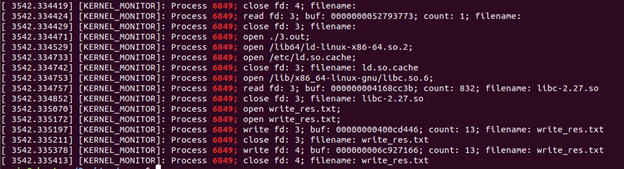
\includegraphics[width = 0.7 \textwidth]{lab_03_3out.png}
        \caption{Пример работы загружаемого модуля ядра.}
        \label{3out}
    \end{figure}

\section{Вывод}
    В данном разделе был обоснован выбор языка программирования, 
    рассмотрены листинги реализованных функций. 
    Приведены результаты работы ПО.

\pagebreak
	\chapter{Исследовательский раздел}
\section{Технические характеристики системы}
Исследование поведения системных функций проводилось
на ноутбуке с процессором Intel(R) Core(TM) i5-7200U CPU 2.50 GHz
в виртуальной машине VmWare c 8 гб оперативной памяти под управлением 
операционной системы Linux (дистрибутив Ubuntu 18.04 x86-64, ядро версии 5.0).

\section{Результаты мониторинга процессов}
    % Для исследования поведения перехватываемых системных вызовов в операционной системе Linux
    % был разработан набор приложений, работающие с файлами.
    % \begin{enumerate}
    %     \item Простейшая программа, которая запускается и сразу завершается.
    %     \item Программа, которая открывает первый файл, потом второй и закрывает первый, затем второй.
    %     \item Программа, которая считывает из файла 10 байт.
    %     \item Программа, которая записывает в файл 10 байт.
    %     \item Многопоточная программа, которая записывает в файл 26 байт с потерей данных.
    % \end{enumerate}
    % \subsection*{1) Программа действий не выполняет:}
    1) Программа никаких действий не выполняет (листинг \ref{lst:example:1})
        \begin{lstlisting}[language=C, label=lst:example:1, caption=Программа не выполняющая никаких действий]
int main()
{
    return 0;
}
        \end{lstlisting}

        Система запускает процесс, который ничего не выполняет.
        На рисунке \ref{examples:1out} представлен результат мониторинга системных вызовов
        выполняемых в ходе работы программы.
        
        \begin{figure}[h!]
            \centering
            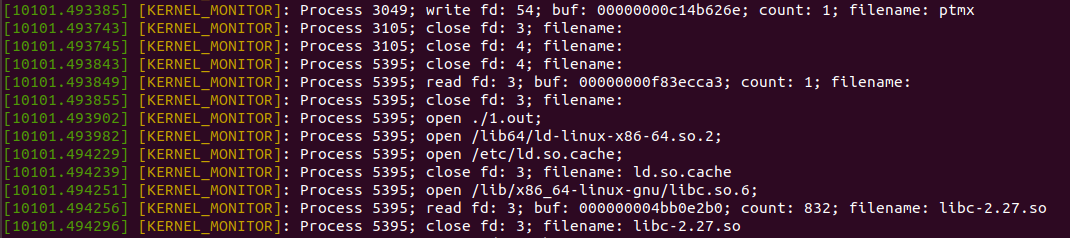
\includegraphics[width = 0.7 \textwidth]{1out.png}
            \caption{Результат мониторинга программы не выполняющей никаких действий.}
            \label{examples:1out}
        \end{figure}

        Из рисунка \ref{examples:1out} видно, что процессы с идентификаторами 3105 (терминал из которого производился запуск программы)
        и 5395 (новый процесс созданный под выполнение программы)
        производят некоторые действия перед открытием исполняемого файла 1.out,
        одно из которых вызовов системного вызова fork для создания процесса программы.
        К сожалению, у некоторых файлов не указывается имя,
        поэтому сложно сказать, какие именно действия производятся 
        %(ниже будет показано, что для других файлов их имена определяются корректно)
        После открытия исполняемого файла происходит загрузка библиотек
        необходимых для работы программы и выполнение кода программы.

        Можно заметить, что не была вызвана функция-обёртка системного вызова
        sys\_open, а только do\_filp\_open, что может быть связано с ассемблерной оптимизацией данного 
        обработчика системного вызова, описанной в аналитическом разделе.

    2) Запускается та же программа (листинг \ref{lst:example:1}),
        но в загружаемый модуль ядра для дополнительного 
        логирования, было добавлено 
        логирование системного вызова get\_unused\_fd\_flags, используя ftrace.

        Из рисунка \ref{examples:1out:alt} видно, что
        файл с исходным кодом 
        открывается с помощью функции do\_filp\_open, а не sys\_open,
        что объясняет отсутствие в лог файле записи о его чтении и закрытии.

        \begin{figure}[h!]
            \centering
            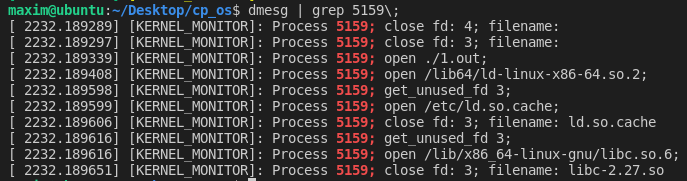
\includegraphics[width = 0.7 \textwidth]{1out-get-fd.png}
            \caption{Результат мониторинга программы не выполняющей никаких действий c дополнительной информацией об открываемом файловом дескрипторе.}
            \label{examples:1out:alt}
        \end{figure}

    3) Программа открывающая и закрывающая файлы (листинг \ref{lst:example:2}).
        \begin{lstlisting}[language=C, label=lst:example:2, caption=Программа открывающая и закрывающая файлы]
#include <fcntl.h>

int main()
{
    int fd1 = open("alphabet.txt", O_RDONLY);
    int fd2 = open("test.txt", O_RDONLY);

    close(fd1);
    close(fd2);
    return 0;
}
        \end{lstlisting}
       
        Система запускает процесс, который открывает существующие файлы alphabet.txt и test.txt,
        после чего закрывает файлы в порядке их открытия.
        
        На рисунке \ref{examples:2out} представлен результат мониторинга системных вызовов,
        выполняемых в ходе работы данной программы.

        Первые 12 строк инициализации процесса были рассмотрены выше.
        Из последних четырёх можно сделать вывод, что
        open возвращает наименьший свободный файловый дескриптор и
        первые три файловых дескрипторов изначально заняты под stdin, stdout, stderr,
        а также корректность определения имени файла по его файловому дескриптору.

        \begin{figure}[h!]
            \centering
            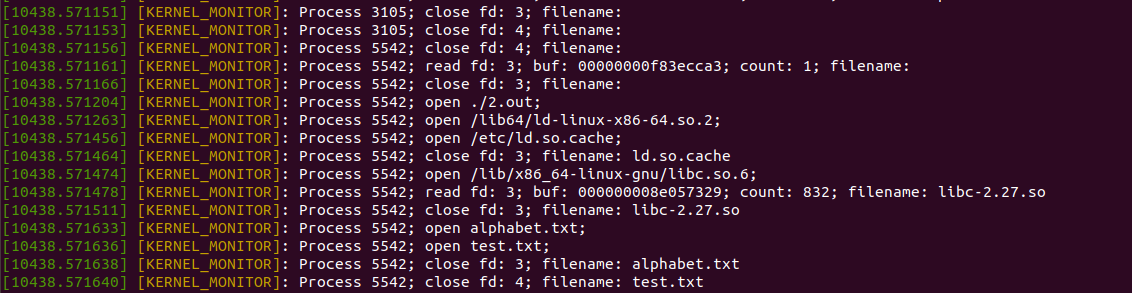
\includegraphics[width = 0.7 \textwidth]{2out.png}
            \caption{Результат мониторинга программы открывающей и закрывающей файлы.}
            \label{examples:2out}
        \end{figure}

    4) Программа с небуферизованным вводом данных (листинг \ref{lst:example:3:alt}).
        \begin{lstlisting}[language=C, label=lst:example:3:alt, caption=Программа с небуфферизованным вводом данных из файла]
#include <fcntl.h>
int main()
{
    int fd = open("alphabet.txt", O_RDONLY);
    char buf[128];

    int len = read(fd, buf, 128);
    buf[len] = 0;
    write(1, buf, len);

    close(fd);
    return 0;
}
        \end{lstlisting}
        
        Система запускает процесс, который открывает существующий файл alphabet.txt
        читает информацию из него, используя системный вызов read, после чего файл закрывается.

        На рисунке \ref{examples:3out:alt} представлен результат мониторинга системных вызовов
        выполняемых в ходе работы данной программы.
        Из рисунка \ref{examples:3out:alt} видно, что небуферизованный ввод использует ровно один вызов функция sys\_read,
        который пытается прочитать из файла 128 байт из открытого файла.

        \begin{figure}[h!]
            \centering
            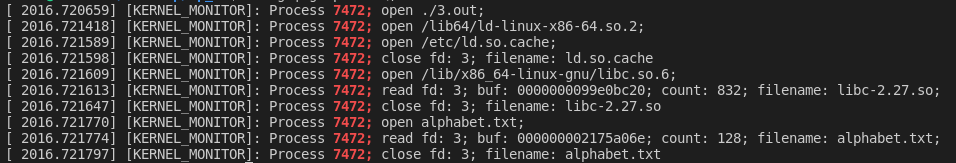
\includegraphics[width = 0.7 \textwidth]{3out-alt.png}
            \caption{Результат мониторинга программы с небуферизованным вводом данных.}
            \label{examples:3out:alt}
        \end{figure}


    5) Программа с буферизованным вводом данных (листинг \ref{lst:example:3}).
        \begin{lstlisting}[language=C, label=lst:example:3, caption=Программа с буфферизованным вводом данных из файла]
#include <stdio.h>

int main()
{
    FILE *f = fopen("alphabet.txt", "r");
    char buf[128];

    fscanf(f, "%s", buf);
    printf("%s", buf);

    fclose(f);
    return 0;
}
        \end{lstlisting}

        Система запускает процесс, который открывает существующий файл alphabet.txt и
        читает информацию из него, используя для этого функцию fscanf
        библиотеки буферизованного ввода/вывода stdio, 
        после чего файл закрывается.

        На рисунке \ref{examples:3out} 
        представлены результаты мониторинга системных вызовов
        выполняемых в ходе работы данной программы.
        
        Из рисунка \ref{examples:3out} видно, что программа с буферизованным вводом дважды
        вызывает системный вызов sys\_read для заполнения буфера размером 4096 байт.

        \begin{figure}[h!]
            \centering
            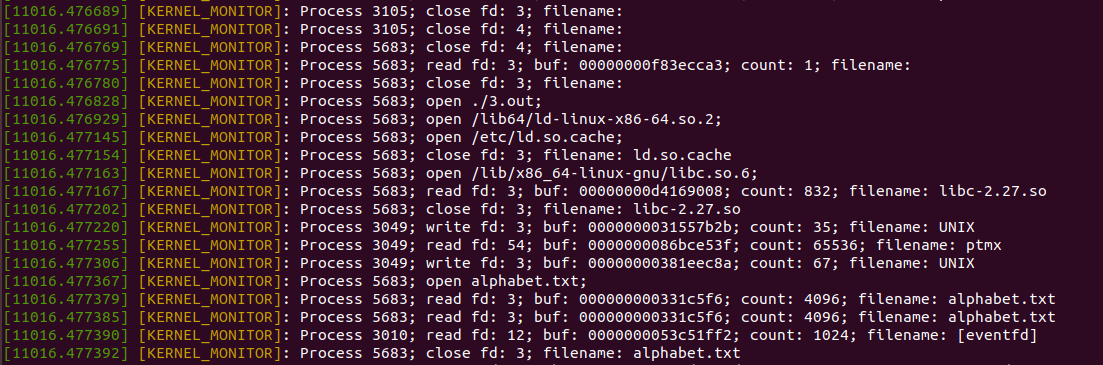
\includegraphics[width = 0.7 \textwidth]{3out.png}
            \caption{Результат мониторинга программы с буферизованным вводом данных.}
            \label{examples:3out}
        \end{figure}

    6) Программа, которая записывает информацию в файл, используя библиотеку буферизованного ввода/вывода (листинг \ref{lst:example:4}).
        \begin{lstlisting}[language=C, label=lst:example:4, caption=Программа с буферизованным выводом данных в файл]
#include <stdio.h>

int main()
{
    FILE *f = fopen("test.txt", "w");
    char buf[128] = "1234567890";
    fprintf(f, "%s", buf);
    fprintf(f, "%s", buf);
    fclose(f);
    return 0;
}
        \end{lstlisting}

        Система запускает процесс, который открывает файл test.txt и
        два раза записывает в него по 10 байт, используя для этого функцию fprintf
        библиотеки буферизованного ввода/вывода stdio, 
        после чего файл закрывается.

        На рисунке \ref{examples:4out} представлен результат мониторинга системных вызовов
        выполняемых в ходе работы данной программы, из которого видно, 
        что системный вызов sys\_write был вызван единожды на запись 20 байт,
        т.к. использовался буфер на 4096 байт, который записывается в файл, 
        либо если буфер полностью заполнен, либо файл закрывается.

        \begin{figure}[h!]
            \centering
            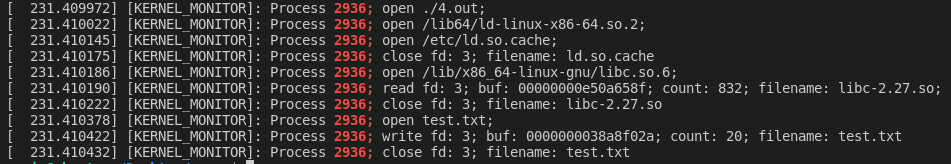
\includegraphics[width = 0.7 \textwidth]{4out-alt.png}
            \caption{Результат мониторинга программы с буферизованным вывод данных.}
            \label{examples:4out}
        \end{figure}

    7) Многопоточная программа, которая записывает в файл с потерей данных (листинг \ref{lst:example:5}).        
        \begin{lstlisting}[language=C, label=lst:example:5, caption=Многопоточная программа записывающая данные в один файл]
#include <stdio.h>
#include <sys/stat.h>
#include <pthread.h>

#define THREADS 4
void *write_file(void *arg)
{
    int num = (int)arg;
    struct stat statbuf;
    FILE *f = fopen("write_thread.txt", "w");

    for (char c = 'a' + num; c <= 'z'; c += THREADS)
        fprintf(f, "%c", c);

    fclose(f);
    return 0;   
}

int main()
{
    pthread_t threads[THREADS];

    for (int i = 0; i < THREADS; i++) 
    {
        int code = pthread_create(threads + i, NULL, write_file, i);
        if (code != 0)
        {
            printf("can't create thread, code = %d\n", code);
            return code;
        }
    }
    
    for (int i = 0; i < THREADS; i++) 
        pthread_join(threads[i], NULL);
    return 0;
}
        \end{lstlisting}

        Проанализируем поведение перехватываемых функций, в случае многопоточной обработки файла.
        Для этого была реализована пятая программа ,
        которая в несколько потоков записывает данные в один файл с потерей данных.

        Система запускает процесс, который в четыре потока,
        открывает файл write\_thread.txt  и записывает в него информацию с потерей данных.
        
        На рисунке \ref{examples:5out} представлен отфильтрованный результат мониторинга системных вызовов
        выполняемых в ходе работы данной программы.
        Из него можно сделать вывод, что потоки в линуксе на самом деле реализованы в виде процессов.

    \begin{figure}[h!]
        \centering
        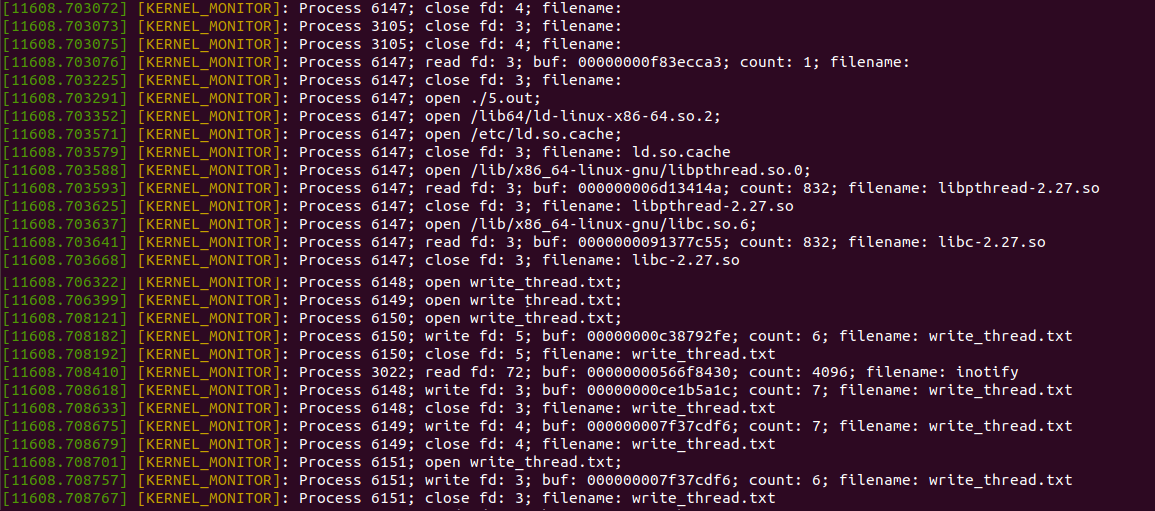
\includegraphics[width = 0.7 \textwidth]{5out-alt.png}
        \caption{Результат мониторинга многопоточной программы записывающая данные в файл с потерей данных.}
        \label{examples:5out}
    \end{figure}

\pagebreak

	\backmatter % Здесь заканчивается нумерованная часть документа и начинаются ссылки и
	\Conclusion
    В соответствии с заданием на курсовую работу по операционным системам
    был реализован загружаемый модуль ядра операционной системы Linux.
    В процессе разработки был реализовать метод, 
    позволяющий перехватить необходимые функции и системные вызовы, 
    и логировать необходимую информацию без перехода в режим пользователя.
    Реализуемый модуль поддерживает ядра версий 5.0 для архитектуры x86\_64.

    Исследованы особенности системных вызовов осуществляющих взаимодеиствие с файловыми системами и
    различными функциями пространства пользователя для буферизованного и небуферизованного ввода/вывода.
    
    Обнаружены файлы, которые не имеют символического имени
    и выявлена проблема с перехватом sys\_open через таблицу системных вызов sys\_call\_table, 
    что может быть связано с ассемблерной оптимизацией данного 
    обработчика системного вызова.
    
    Показано, что библиотека для работы с потоками в операционной системе Linux,
    на самом деле создаёт процессы, т.к. потоки в Linux <<дорогие>>.

\pagebreak
	% % Список литературы при помощи BibTeX
% Юзать так:
%
% pdflatex report
% bibtex report
% pdflatex report

\bibliographystyle{gost780u}
\bibliography{rpz}

\pagebreak

	\appendix % Тут идут приложения
	\chapter{Диаграмма }
\label{chapter:appendix:1}

\pagebreak
\end{document}
